\documentclass[border=6pt]{standalone}
\usepackage[T1]{fontenc}
\usepackage{courier}
\usepackage[scaled=0.95]{helvet}
\renewcommand{\familydefault}{\sfdefault}
\usepackage{sfmath}
\usepackage[version=4]{mhchem}
\usepackage{tikz}
\usepackage{pgfplots}
\pgfplotsset{compat=newest}
\usetikzlibrary{arrows.meta,positioning,calc,fit,backgrounds,shapes.geometric,decorations.pathreplacing,patterns}
\definecolor{ink}{HTML}{17233A}
\definecolor{inksoft}{HTML}{44506A}
\definecolor{teal}{HTML}{0E6B6B}
\definecolor{tealsoft}{HTML}{E5F0EF}
\definecolor{amber}{HTML}{B26B12}
\definecolor{ambersoft}{HTML}{FBF0DF}
\definecolor{blue}{HTML}{2F6690}
\definecolor{bluesoft}{HTML}{E3ECF4}
\definecolor{plum}{HTML}{7A4D8C}
\definecolor{plumsoft}{HTML}{EFE7F3}
\definecolor{greyc}{HTML}{8A94A3}
\definecolor{linec}{HTML}{D3DCE1}
\definecolor{oxy}{HTML}{C0392B}
\definecolor{carb}{HTML}{3B4252}
\definecolor{hyd}{HTML}{E6E9EE}
\definecolor{nit}{HTML}{2F6690}
\tikzset{
  every picture/.style={line cap=round,line join=round},
  lab/.style={font=\small, text=inksoft},
  >={Stealth[length=7pt]},
}
\pgfplotsset{
  every axis/.append style={axis line style={inksoft}, tick style={inksoft}, tick label style={font=\footnotesize, text=inksoft}, label style={font=\small, text=ink}},
}
% fragment tile: \frag{node name}{position}{colour}{content}
\newcommand{\frag}[4]{\node[draw=#3, fill=#3!12, line width=1.4pt, rounded corners=6pt, minimum width=1.25cm, minimum height=1.05cm, text=#3, font=\bfseries] (#1) at (#2) {#4};}
\newcommand{\ring}{\tikz[baseline=-0.6ex]{\draw[line width=1.1pt] (0:0.3)--(60:0.3)--(120:0.3)--(180:0.3)--(240:0.3)--(300:0.3)--cycle; \draw[line width=0.8pt] (0,0) circle (0.16);}}
\newcommand{\bond}[2]{\draw[ink, line width=2.2pt] (#1) -- (#2);}

\begin{document}
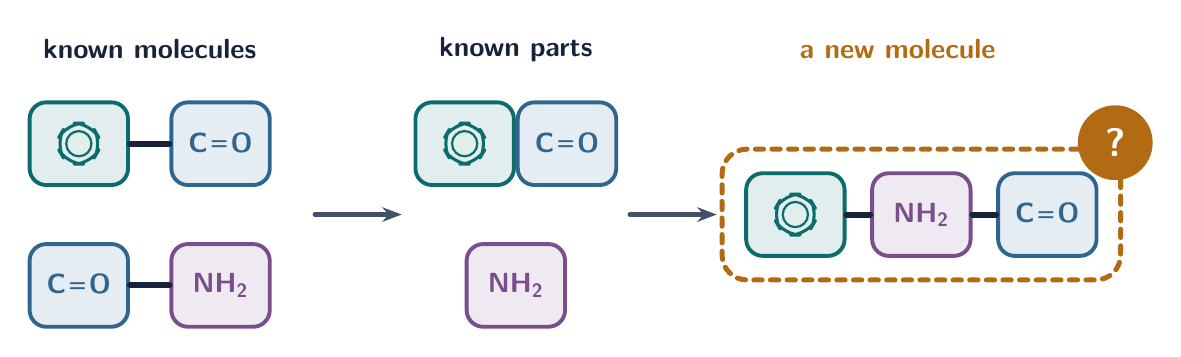
\begin{tikzpicture}
\node[font=\bfseries, text=ink] at (1.5,3.4) {known molecules};
\frag{a1}{0.6,2.2}{teal}{\ring}\frag{b1}{2.4,2.2}{blue}{\ce{C=O}}\bond{a1}{b1}
\frag{b2}{0.6,0.4}{blue}{\ce{C=O}}\frag{c2}{2.4,0.4}{plum}{\ce{NH2}}\bond{b2}{c2}
\draw[->, inksoft, line width=1.8pt] (3.6,1.3) -- (4.7,1.3);
\node[font=\bfseries, text=ink] at (6.15,3.4) {known parts};
\frag{a}{5.5,2.2}{teal}{\ring}\frag{b}{6.8,2.2}{blue}{\ce{C=O}}\frag{c}{6.15,0.4}{plum}{\ce{NH2}}
\draw[->, inksoft, line width=1.8pt] (7.6,1.3) -- (8.7,1.3);
\node[font=\bfseries, text=amber] at (11.0,3.4) {a new molecule};
\frag{a3}{9.7,1.3}{teal}{\ring}\frag{c3}{11.3,1.3}{plum}{\ce{NH2}}\frag{b3}{12.9,1.3}{blue}{\ce{C=O}}\bond{a3}{c3}\bond{c3}{b3}
\node[draw=amber, line width=1.8pt, dashed, rounded corners=9pt, fit=(a3)(b3), inner sep=8pt] (nb) {};
\node[circle, fill=amber, text=white, font=\Large\bfseries, minimum size=0.95cm] at ($(nb.north east)+(-0.1,0.05)$) {?};
\end{tikzpicture}
\end{document}
